\documentclass[a4paper,12pt]{article}
\usepackage[utf8]{inputenc}
\usepackage[english]{babel}
\usepackage[T1]{fontenc}
\usepackage{amsmath}
\usepackage{amssymb}
\usepackage{graphicx}
\title{Snake-AI\\Project Documentation}
\author{Ibrahim Enes Hayber, Rana MD Jewel, Maximilian Lüttich\\
		Frankfurt University of Applied Sciences\\
		Faculty 2, Computer Science (B. Sc.)\\
		Object-oriented Programming in Java by Prof. Dr. Doina Logofatu
}

\date{\today}

\begin{document}

\maketitle
\newpage
\tableofcontents
\newpage

\section{How we started}

This chapter describes how we started with the project.\\
\\As we all know the hardest part of a journey is the start. But once started it is a easy on going.
It is like the starting impact on the first domino stone, which brings the whole project in rolling.
\\As usual in any task of life we need to understand what the problem is and which requirements are necessary to solve the problem. To do so, we read the description from the organizers carefully. In addition to that we watched a few videos about our topic to get a better understanding.\\
After gaining knowledge about the problem we felt ready to start working with the Snake-AI project provided by the organizers on a GitHub repository. The Project was written in the Java programming language. To get familiar with the project we looked into the UML class
diagram. Besides that we followed a YouTube Tutorial which was also provided by the organizers, where we implemented our first working version. A detailed introduction and our results will now be presented.
\newpage

\section{Introduction}
to-do
\subsection{General Topic}
to-do
\subsection{Similar problems in practice (References every time, look for actual ones)}
to-do

\section{Team Work}
to-do
\subsection{Work Participation}
to-do

\subsection{work structure (communication, decisions, bug tracking, repository, engineering, ...)}
to-do

\subsection{ideas (brainstorming)}
to-do

\section{Problem Description}
to-do
\subsection{Formal description: definitions, examples, ...}
to-do
jflafjlajflajfla
\section{Related Work}
to-do
\subsection{Related Algorithms, Applications}
to-do

!for example: Fractals, Data Generation, Games, Evolutionary Algorithms (Genetic Algortihms; Collective Intelligence like Particle Swarm Optimization - PSO, Ant Colony Optimizaton - ACO; Evolutionary Multiobjective Optimization, ...)

\section{Proposed Approaches}
to-do
\subsection{Input/Output Format, Benchmarks (Generation, Examples)}
to-do
\subsection{Algorithms in Pseudocode}
to-do

\section{Implementation Details}
 this is my test
to-do
\subsection{Application Structure}
The Snake AI project consists of one Interface, one Enum and eight classes. They are following, 

\begin{itemize}
\item Bot(Interface)
\item Direction(Enum)
\item BotLoader
\item Coordinate
\item Snake
\item SnakeGame
\item SnakeCanvas
\item SnakesRunner
\item SnakeUIMain
\item SnakesWindow
\end{itemize}

\subsection{GUI Details}
In this section all the classes will be discussed in details. 
\subsubsection{SnakeUIMain}
This class is the Entry point of the UI and implements tournament of the Snake game with several rounds. The main method of the class gets two classes(snake \& opponent) implementing the Bot interface as arguments. The class is also responsible to launch several rounds of snake game between bots. In this class the basic I/O actions are performed to record scores of opponent, apple eaten by both the snakes and time taken in each rounds which will be later used to make further statistical analysis.
\subsubsection{BotLoader}
The class BoatLoader fetches the class given the name  of the class and package. The class is taken from the classpath and could be dynamically added after the game of the Bot class. This class inharites the abstrack Java class ClassLoader.\\
A class loader is an object that is responsible for loading classes. The class ClassLoader is an abstract class. Given the binary name of a class, a class loader should attempt to locate or generate data that constitutes a definition for the class. A typical strategy is to transform the name into a file name and then read a "class file" of that name from a file system.%\cite{shafiei2012modeling to-do}
(to-do code snippet)
\\
The only method of BotLoader class gets classBinName as argument and returns an instance of the Bot class.

\subsubsection{SnakesWindow}
This class is responsible for the game's GUI window. The class creates and set ups the window and runs the UI. At the end it closes the frame. This class implements Runnable.\\
The Runnable interface should be implemented by any class whose instances are intended to be executed by a thread. The class must define a method of no arguments called run.\\
This interface is designed to provide a common protocol for objects that wish to execute code while they are active. For example, Runnable is implemented by class Thread. Being active simply means that a thread has been started and has not yet been stopped.\\
In addition, Runnable provides the means for a class to be active while not subclassing Thread. A class that implements Runnable can run without subclassing Thread by instantiating a Thread instance and passing itself in as the target. In most cases, the Runnable interface should be used if you are only planning to override the run() method and no other Thread methods. This is important because classes should not be subclassed unless the programmer intends on modifying or enhancing the fundamental behavior of the class.(to-do ref)
\subsubsection{SnakesRunner}
This class also implements Runnable interface and is used for running bots in a separate threads. The Constructor of the class SnakesRunner recieves running bot, snake that is controlled by the current bot, opponent's snake, size of the board and coordinate of the current apple as arguments. In addition the chooseDirection method of the current bot is executed and saved(current direction) by this class. 
\subsubsection{SnakesGame}
The class SnakesGame implements the main games flow and runs game for two bots. The Override toString() method converts the game to string representation and return game state as a string. randomNonOccupiedCell() method selects random non-occupied cell of maze which is used to create new location of a apple. If a Snake takes more than one seconds to choose its  next direction the runOneStep() methods stopps that rounds.

\subsubsection{SnakeCanvas}
The purpose of this class is to design the UI and give the UI a better look. This class helps to fill the  snake Body wicht color and make it visible on the UI. After filling the body of snake and opponent and apple the render() method renders the game. After every movement of the snake, opponent and apple the previous occupied positions are recolord and marked the free for next movement. This class inharites the Java swing class JPanel which is used to create different generic lightweight container with one or more single component.
\subsubsection{Snake}
This class implements snake body(not brain) that determines the place of head, body, and length of body on the game board. For implementing the body of the snake two logical and efficient data structure from Java Collections framework are used. They are,
\begin{itemize}
\item Dequeue
\item HashSet
\end{itemize}
Deque(double ended queue) data structure helps to add or delete elements from both side(head and tail) within $\mathcal{O}(1)$ constant time coplexity. On the other hand HashSet data structure ensures basics search operation in $\mathcal{O}(1)$ time complexity.\\
This class has a important feature of cloneability which allows to copy one object to another object without using new operator.\\
A class implements the Cloneable interface to indicate to the Object.clone() method that it is legal for that method to make a field-for-field copy of instances of that class.
Invoking Object's clone method on an instance that does not implement the Cloneable interface results in the exception CloneNotSupportedException being thrown.(to-do ref)
\subsubsection{Coordinate}
Coordinates class implements position of a cell on the game board. It helps to grow up the snake by adding new coordinate at the beginning of the snake body. inBounds() methods helps to keep the snake in side the game board. This methods implements Comparable interface which is useful while comparing two Coordinate. 
\subsubsection{Bot}
This Interface provides functions that should be implemented to create smart and intelligent snake bot for the game. chooseDirection() methds returns an appropriate next moves which plays a vital role to continue the game. 

\subsection{UML Diagram}

\begin{figure}[h]
\centering
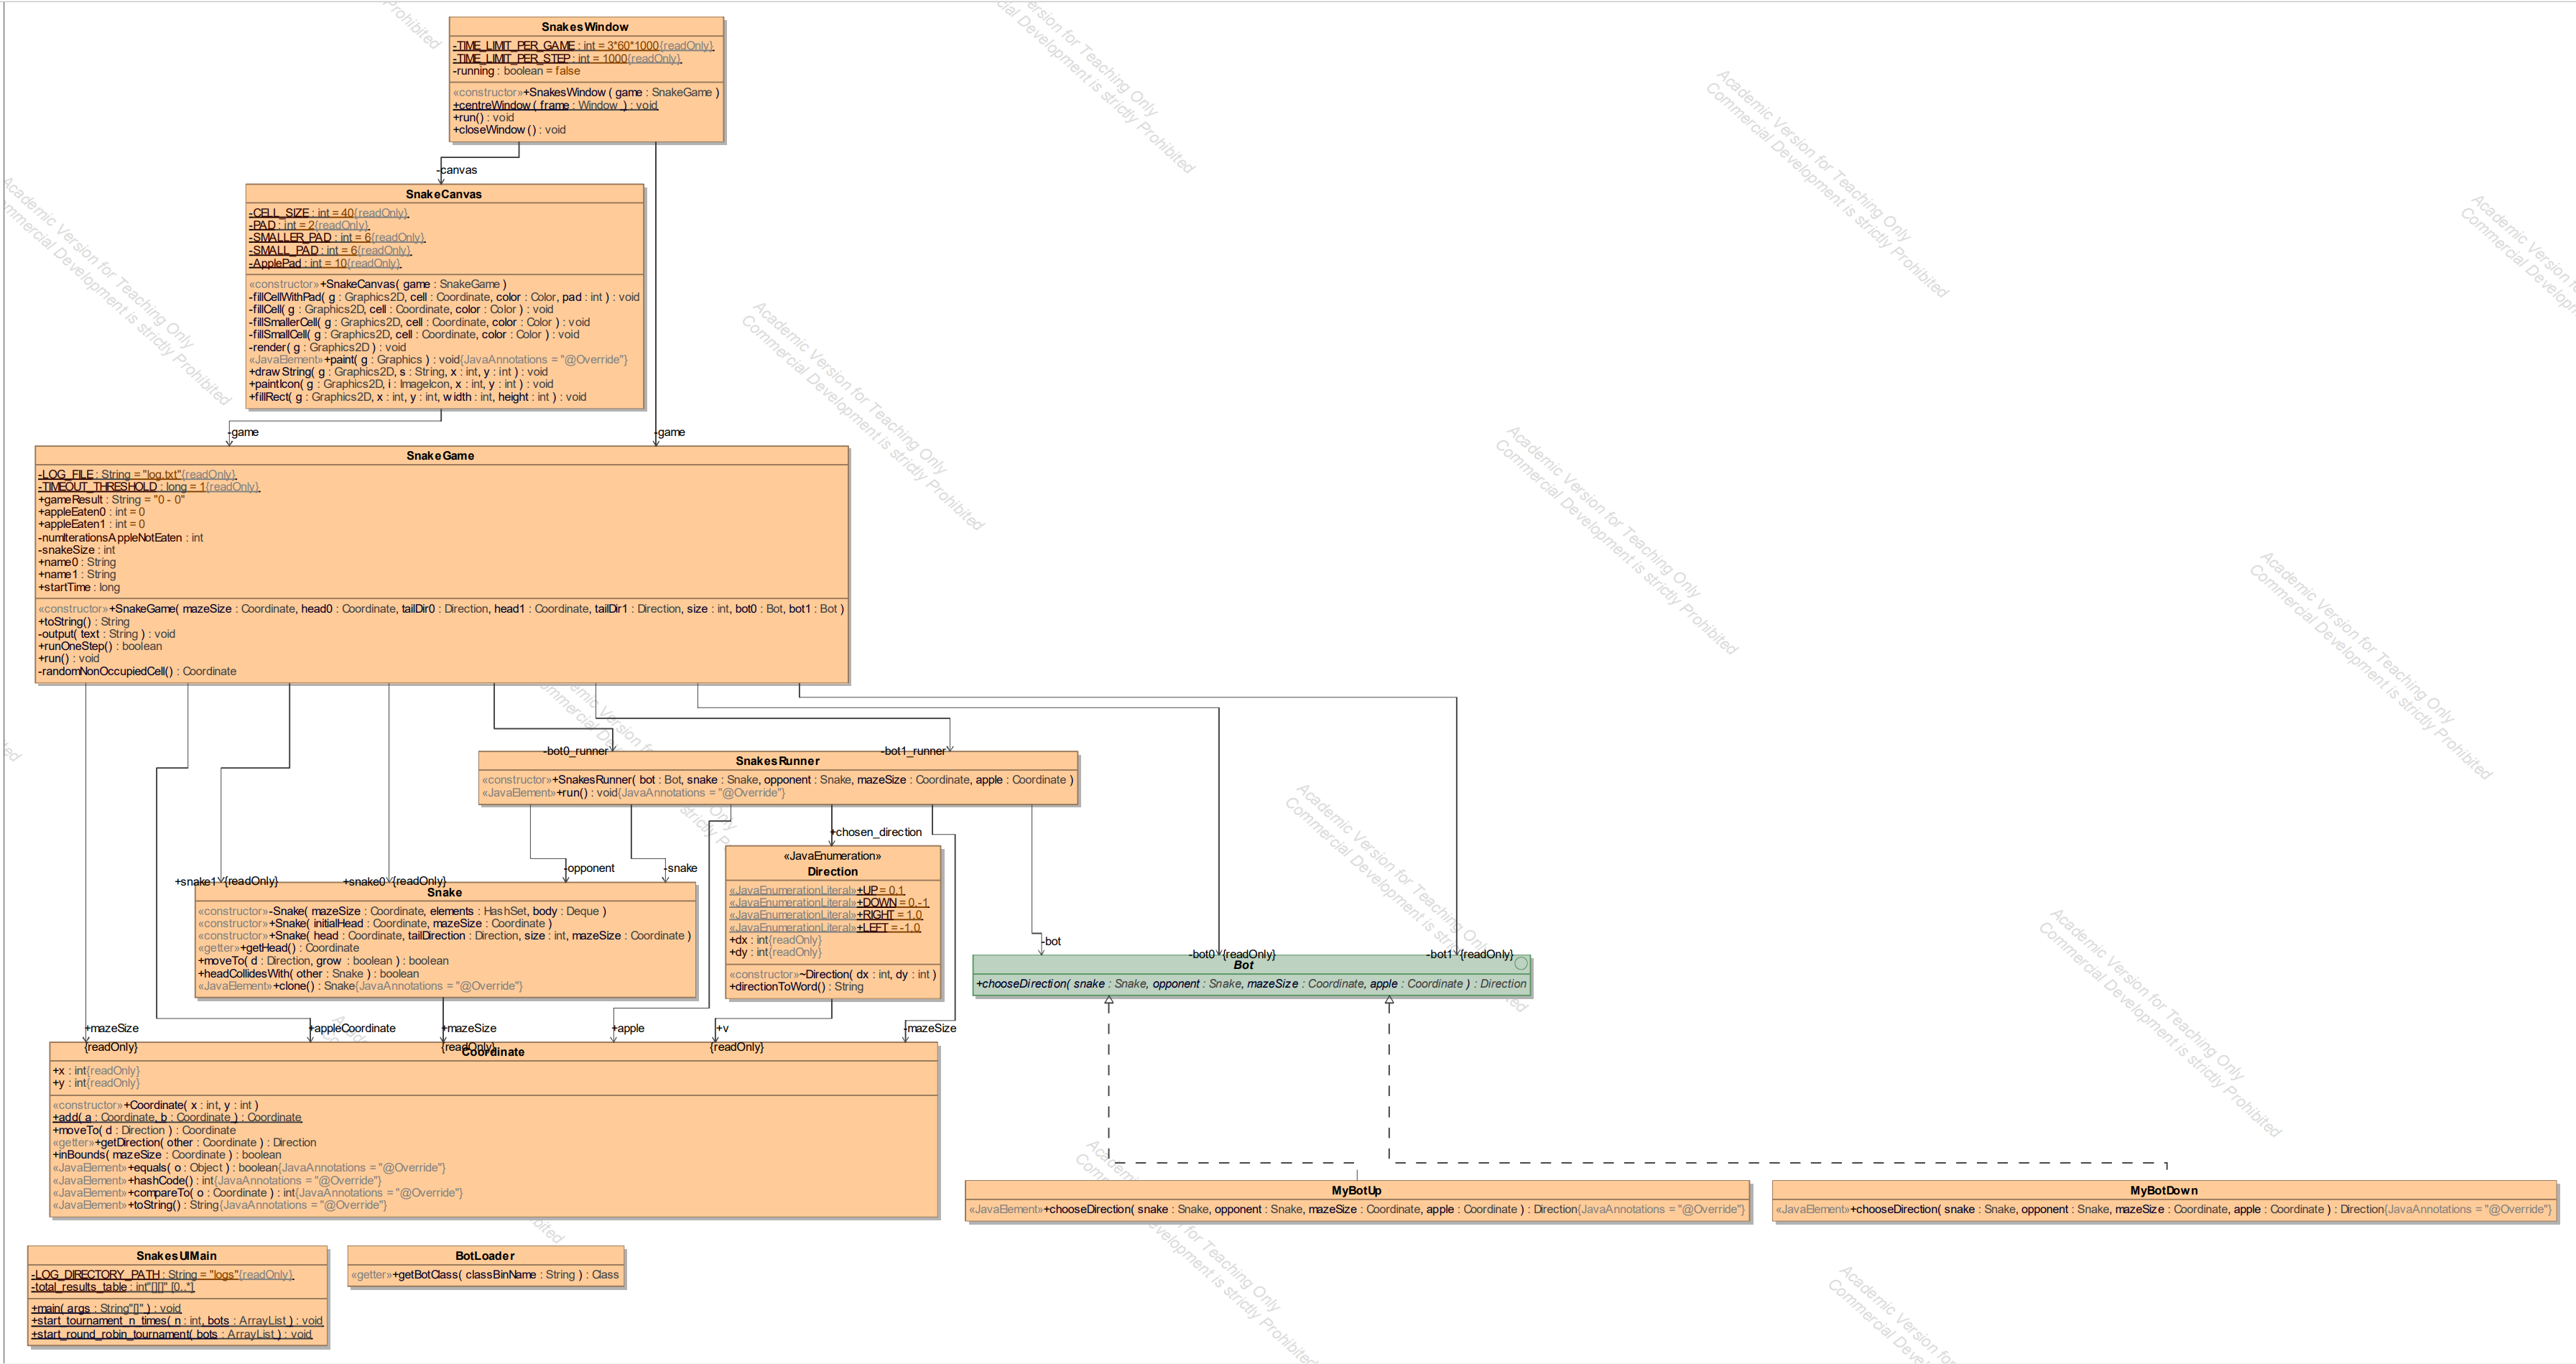
\includegraphics[scale=0.26]{ui.png}
\caption{UML diagram of the GUI}
%\label{fig:abc}
\end{figure}

\subsection{Used Libraries}
For the Developement of the Snake AI Game Java Swing Framework has been used.
Some Components from AWT framework have also been used.\\ 
Swing is a Java Foundation Classes [JFC] library and an extension of the Abstract Window Toolkit [AWT]. Swing offers much-improved functionality over AWT, new components, expanded components features, and excellent event handling with drag-and-drop support.(to-do ref)
 
%\subsection{Code Snippets} write code snippet with discription.


\section{Experimental Results and Statistical Tests}
to-do
\subsection{Simulations (Play with the Parameters!)}
to-do
\subsection{Use Benchmarks}
to-do
\subsection{Tables: input data details, results of different algorithms}
to-do
\subsection{Charts}
to-do
\subsection{Evaluations}
to-do

\section{Conclusions and Future Work}
to-do
\subsection{How the team work went}
to-do
\subsection{What we have learned}
to-do
\subsection{Ideas for the future development of your application, new algorithms}
%to-do\cite{kramer1999api}
%\bibliographystyle{ieeetran}
%\bibliography{myref}
\end{document}